\documentclass[a4paper]{article}
\usepackage{geometry}
 \geometry{
 a4paper,
 total={210mm,297mm},
 left=1.25in,
 right=1.25in,
 top=1.25in,
 bottom=1.25in,
 }
\usepackage{graphicx}
%\usepackage[T1]{fontenc}
%\usepackage{tgpagella}
%\usepackage{todonotes}
%\usepackage{graphicx}
\usepackage{float}
\usepackage{subcaption}
\usepackage[caption = false]{subfig}
\usepackage{amsmath}
\usepackage{amssymb}
\begin{document}

\title{Interactive Foreground Extraction using Iterated Graph Cuts}
\author{Sasank Chilamkurthy\\Tharun Kumar Reddy\\Rajeev Puppala}
\date{\today}
\maketitle

\section{Introduction}
In this report, we describe a method to extract foreground out of a image with help of a very simple interaction from user. This is based on the papers \cite{1} and \cite{2}.

\section{Image Segmentation by Graph Cut}
In this section, general segmentation framework we have used is detailed. Denote the given input image as an array $\bar{z} = (z_1, z_2, \dots z_N)$. 
The segmentation of the image is expressed as an array of "opacity" values $\bar{\alpha} = (\alpha_1, \alpha_2, \dots \alpha_N)$. 
Generally for soft segmentation  $\alpha_n \in [0,1]$ and for hard segmentation $\alpha_n \in \{0,1\}$. 
In this report, we deal with hard segmentation with $0$ representing background and $1$ representing foreground.

Let the model parameters for color/intensity model of the background and foreground be denoted by $\theta_\alpha$ for $\alpha$ equal to $0$ and $1$ respectively. 
Under this model, let likelihood function be given by $f(z|\theta_\alpha)$. Let us denote all the parameters of the model with $\bar{\theta}$.
So, our objective is to find $\bar{\alpha}$ given model parameters $\bar{\theta}$.

This can be achieved by minimizing the following with respect to $\bar{\alpha}$ :
\[ 
E(\bar{\alpha}| \bar{\theta},\bar{z} ) = U(\bar{\alpha}| \bar{\theta},\bar{z}) + V(\bar{\alpha},\bar{z})
\]
Here, 
\[
U(\bar{\alpha}| \bar{\theta},\bar{z}) = \sum_{n=1}^N -\log f(z_i | \theta_{\alpha_i})
\] 
is called data term or unary term. Observe that this is negative log likelihood of the image data $\bar{z}$. The term
\[
V(\bar{\alpha},\bar{z}) = \gamma \sum_{(m,n) \in C} \operatorname{dis}^-1(m,n) \mathbf{1}_{\alpha_m \neq \alpha_n} \exp{-\beta(z_m-z_n)^2}
\]
is called smoothness term with $\beta$ and $\gamma$ suitably chosen constants. $C$ is set of all neighbouring pixels and $\operatorname{dis}(m,n)$ is Euclidean distance between pixel $m$ and $n$.  
This term can be seen as contribution of the prior on $\bar{\alpha}$ that segmentation tends to be smooth. Thus our problem is 
\begin{equation}
\begin{aligned}
& \underset{\bar{\alpha}\in\{0,1 \}^N}{\text{minimize}}
& & E(\bar{\alpha}| \bar{\theta},\bar{z} )
\end{aligned}
\end{equation}

Note that this problem is a discrete optimization problem. 
However, efficient exact solution exists as this problem can be posed in the form of Graph Cuts.
A standard minimum cut algorithm \cite{2,3} can be employed to solve this.

Now that we have seen general framework of segmentation, we'll next discuss the models of the background and foreground we have used.

\section{Background/Foreground Intensity Models}
In this section, we deal with models and estimation of model parameters $\bar{\theta}$. This is where user interaction comes into play. Our user draws a rectangle roughly around the desired foreground. We use this to estimate model parameters.

\subsection{Histograms}
If the image $\bar{z}$ is gray image, then it is conceivable to use histograms as intensity models. Indeed, if we wish to use this model, we convert the input colour image to a gray image and build histograms, one for background and another for foreground. 
However, we will lose discriminatory power color image provides.

\subsection{GMMs}
Unlike above, we cannot hope to build a histogram for three dimensional color data. 
So instead, we fit a Gaussian mixture model of $k$ components to each of the foreground and background. 

\subsection{General Iterative Algorithm}
In the first iteration, model parameters $\bar{\theta}$ are obtained from user supplied rectangle foreground and background. 
These are used to segment the image and this segmentation is in turn used to improve the parameter estimates. This process is repeated until convergence or some maximum iterations are hit.
This is beneficial as our segmentation estimate keeps on improving.
We detail this iterative algorithm:
\begin{description}
\item[1. User Interaction]:
Set $T_1 = \{z_i | i \in \text{user drawn rectangle }\}$ and $T_0 = T_1^c$. 

\item[2. Paramter Estimation]: Estimate parameters $\theta_0$ and $\theta_1$ from $T_0$ and $T_1$ respectively. 

\item[3. Segmentation]: Solve 
\begin{equation*}
\begin{aligned}
\bar{\alpha} &=  
 \underset{\bar{\alpha}\in\{0,1 \}^N}{\text{minimize}}
 & E(\bar{\alpha}| \bar{\theta},\bar{z} )
\end{aligned}
\end{equation*}
and update $T_k = \{z_i | \alpha_i = k\}$, $k = 0,1$

\item[4. Check for Convergence]: If convergence is not reached or maximum iterations is not hit,  
go to step 2. Otherwise return $\alpha$.
\end{description}

\section{Experiments}
We present results from experiments from the above two models.
\subsection{Histogram Model}
Figure 1 shows segmentations for 3 different pictures. 
Although, first two pictures were handled quite easily, last image (parrot) couldn't be handled with this simple model as in gray picture, some parts of parrot looks similar to the background. 
As we will see, this can be handled better if full color data is considered.


\begin{figure}[h]
\begin{subfigure}{.5\textwidth}
  \centering
  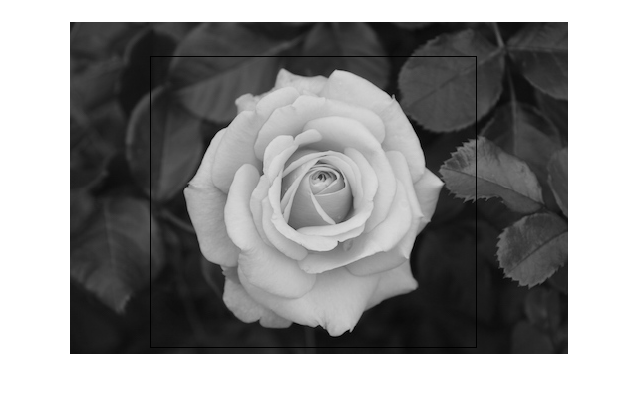
\includegraphics[width = 3in]{rose_input_h.png}
  \label{fig:sfig1}
\end{subfigure}%
\begin{subfigure}{.5\textwidth}
  \centering
  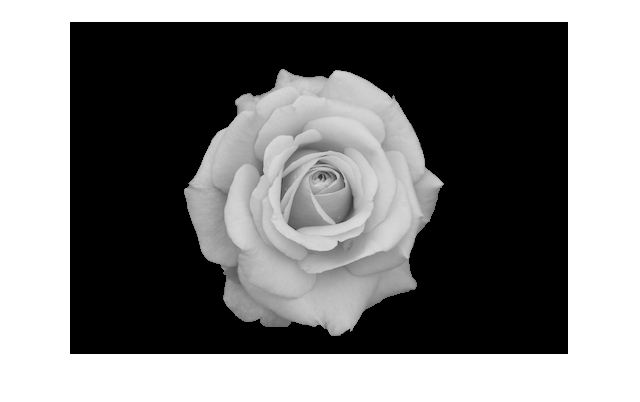
\includegraphics[width = 3in]{rose_output_h.png}
  \label{fig:sfig2}
\end{subfigure}


\begin{subfigure}{.5\textwidth}
  \centering
  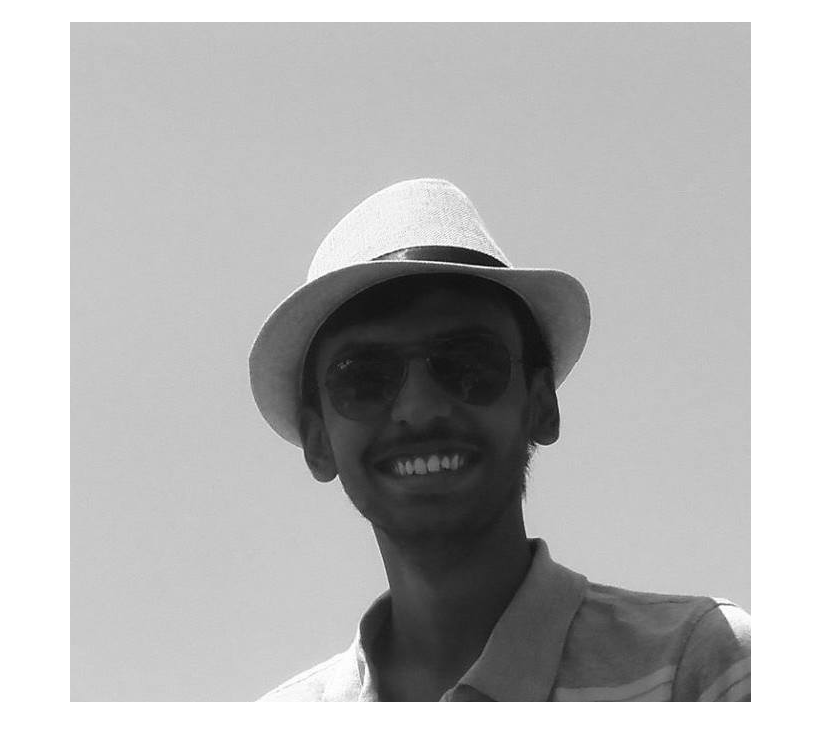
\includegraphics[width = 3in]{varun_input_h.png}
  \label{fig:sfig2}
\end{subfigure}
\begin{subfigure}{.5\textwidth}
  \centering
  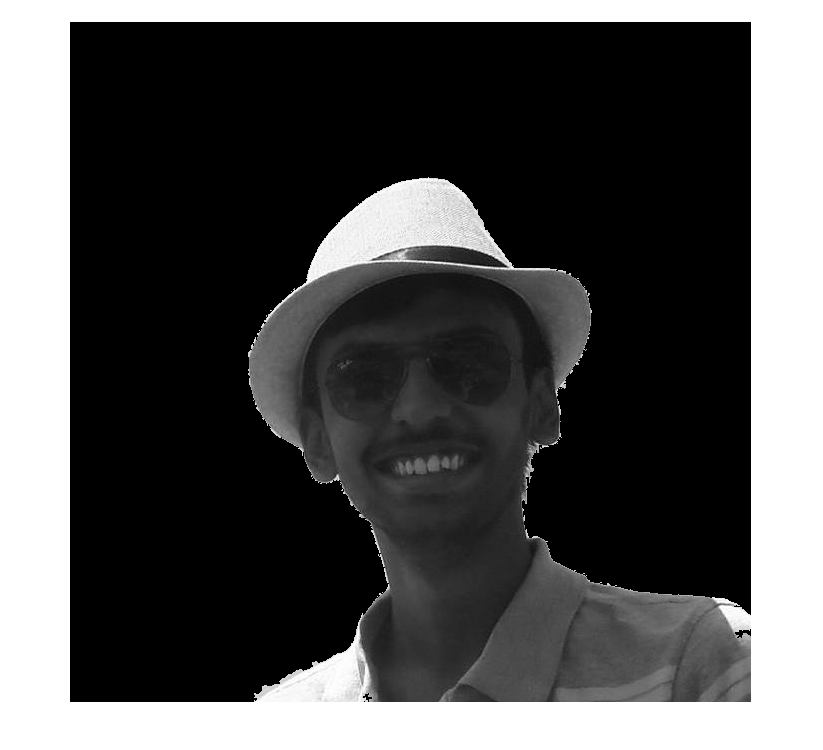
\includegraphics[width = 3in]{varun_output_h.png}
  \label{fig:sfig2}
\end{subfigure}

\begin{subfigure}{.5\textwidth}
  \centering
  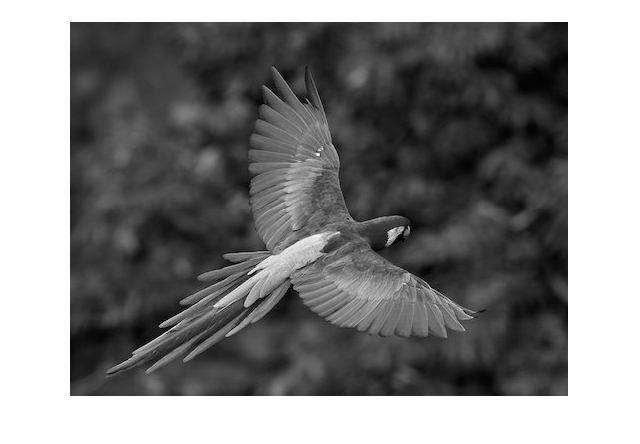
\includegraphics[width = 3in]{parrot_input_h.png}
  \label{fig:sfig2}
\end{subfigure}
\begin{subfigure}{.5\textwidth}
  \centering
  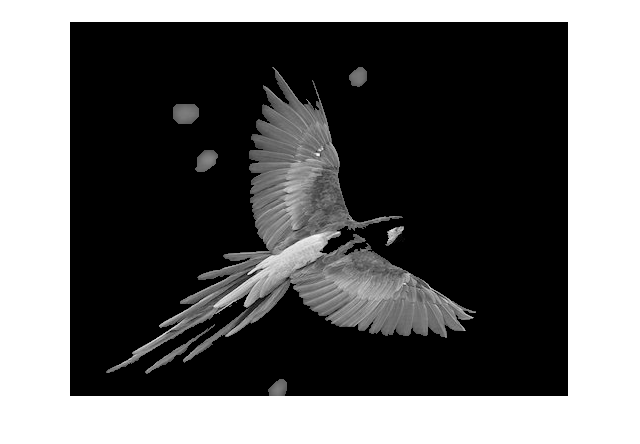
\includegraphics[width = 3in]{parrot_output_h.png}
  \label{fig:sfig2}
\end{subfigure}

\caption{Foreground Extractions for Histogram Model}
\end{figure}

\subsection{GMM Model}
\begin{figure}[h]
\begin{subfigure}{.5\textwidth}
  \centering
  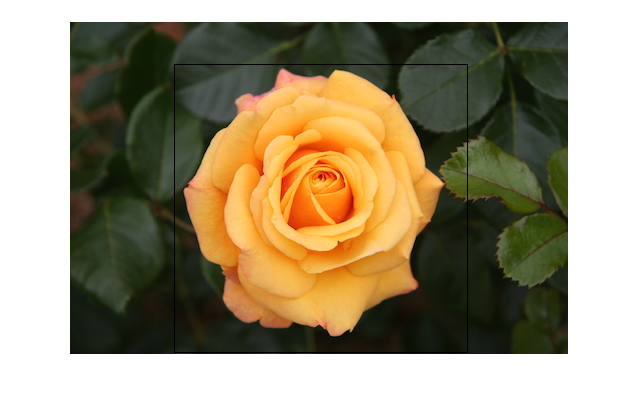
\includegraphics[width = 3in]{rose_input_g.png}
  \label{fig:sfig1}
\end{subfigure}%
\begin{subfigure}{.5\textwidth}
  \centering
  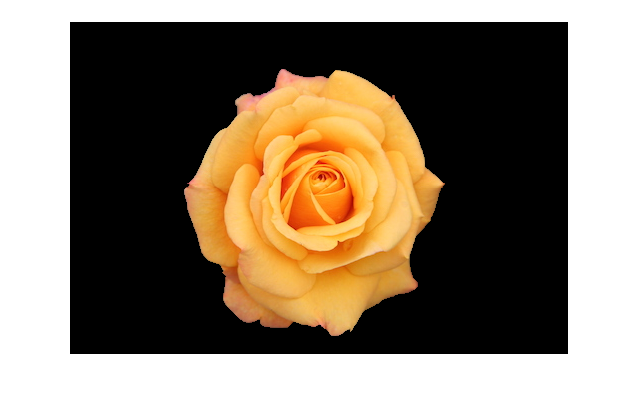
\includegraphics[width = 3in]{rose_output_g.png}
  \label{fig:sfig2}
\end{subfigure}


\begin{subfigure}{.5\textwidth}
  \centering
  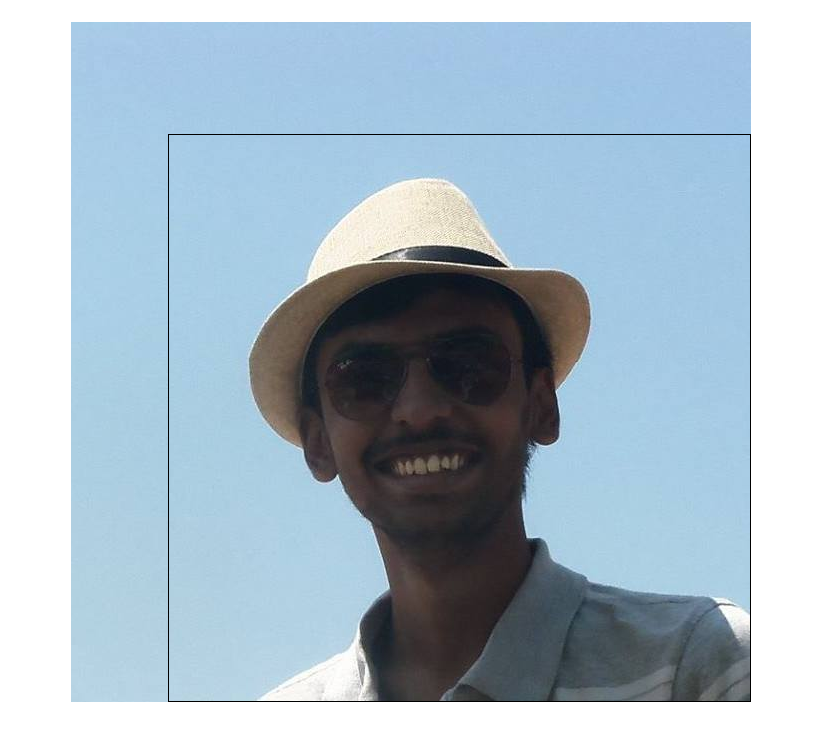
\includegraphics[width = 3in]{varun_input_g.png}
  \label{fig:sfig2}
\end{subfigure}
\begin{subfigure}{.5\textwidth}
  \centering
  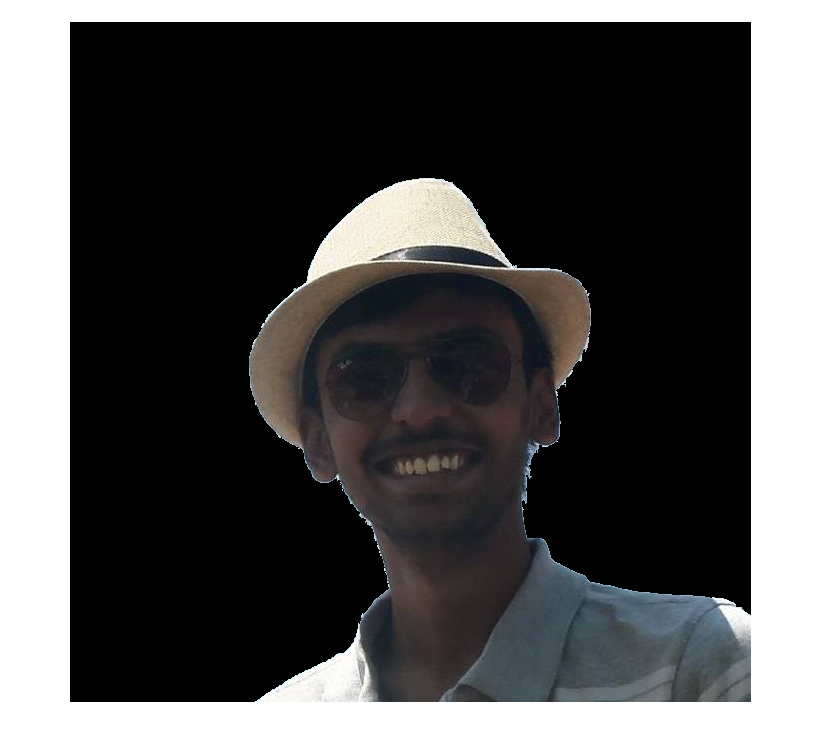
\includegraphics[width = 3in]{varun_output_g.png}
  \label{fig:sfig2}
\end{subfigure}

\begin{subfigure}{.5\textwidth}
  \centering
  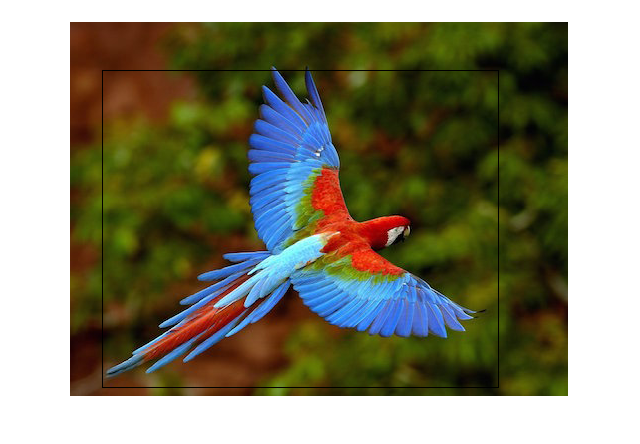
\includegraphics[width = 3in]{parrot_input_g.png}
  \label{fig:sfig2}
\end{subfigure}
\begin{subfigure}{.5\textwidth}
  \centering
  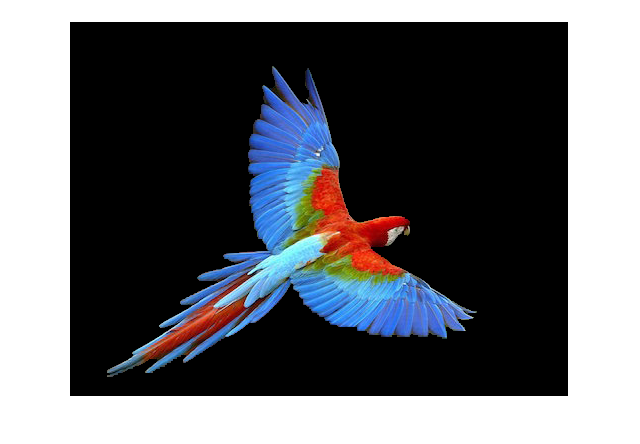
\includegraphics[width = 3in]{parrot_output_g.png}
  \label{fig:sfig2}
\end{subfigure}

\begin{subfigure}{.5\textwidth}
  \centering
  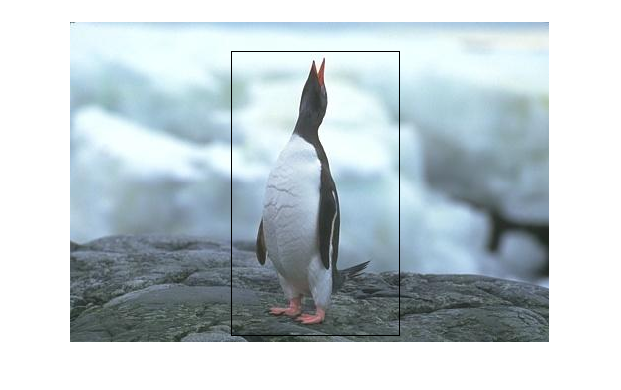
\includegraphics[width = 3in]{penguin_in.png}
  \label{fig:sfig2}
\end{subfigure}
\begin{subfigure}{.5\textwidth}
  \centering
  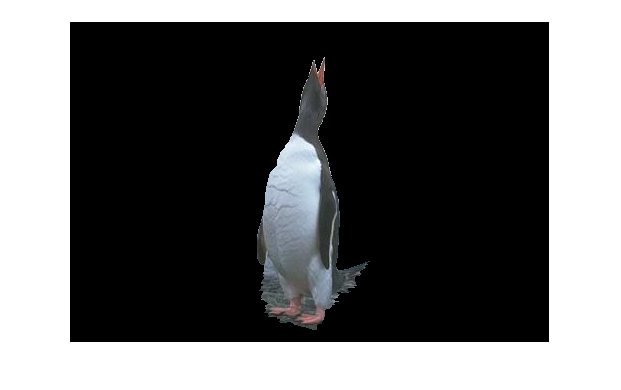
\includegraphics[width = 3in]{penguin_out.png}
  \label{fig:sfig2}
\end{subfigure}

\caption{Foreground Extractions for GMM Model}
\end{figure}

\begin{figure}[h]
\begin{subfigure}{.5\textwidth}
  \centering
  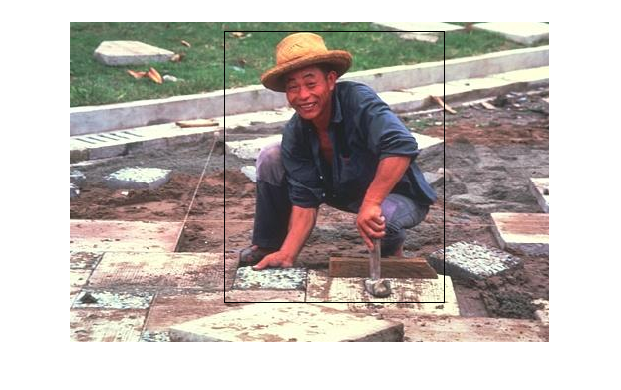
\includegraphics[width = 3in]{man_in.png}
  \label{fig:sfig1}
\end{subfigure}%
\begin{subfigure}{.5\textwidth}
  \centering
  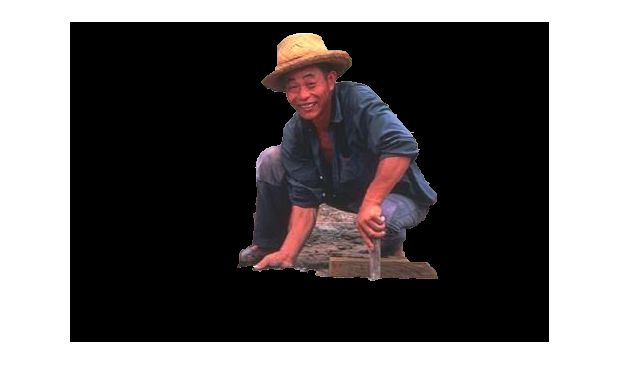
\includegraphics[width = 3in]{man_out.png}
  \label{fig:sfig2}
\end{subfigure}


\begin{subfigure}{.5\textwidth}
  \centering
  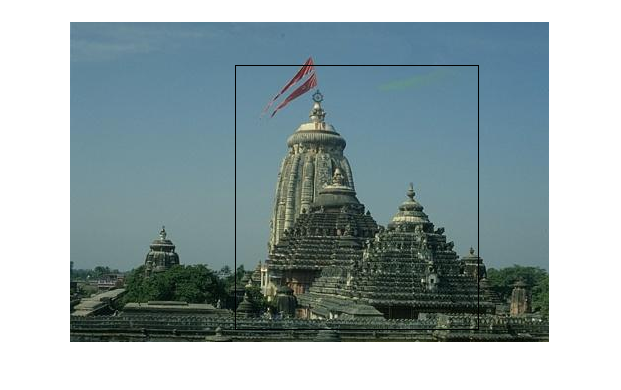
\includegraphics[width = 3in]{temple_in}
  \label{fig:sfig2}
\end{subfigure}
\begin{subfigure}{.5\textwidth}
  \centering
  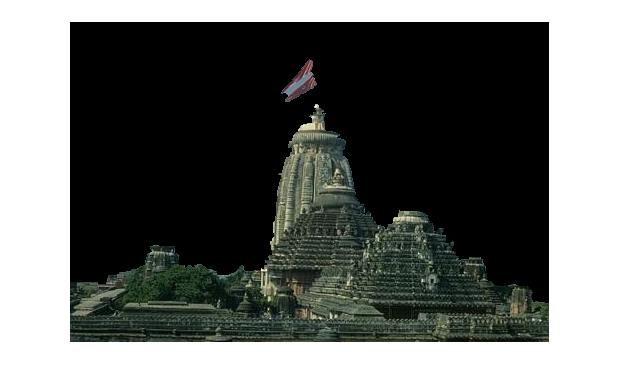
\includegraphics[width = 3in]{temple_out}
  \label{fig:sfig2}
\end{subfigure}

\begin{subfigure}{.5\textwidth}
  \centering
  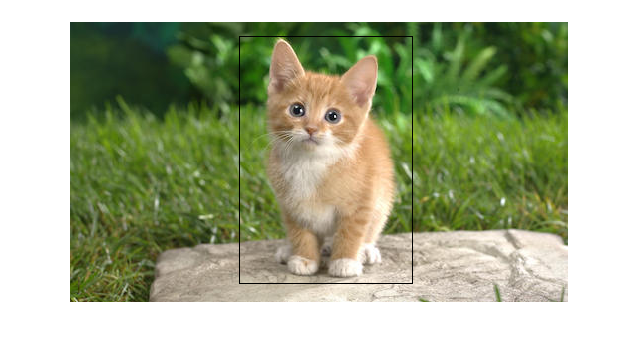
\includegraphics[width = 3in]{cat_in}
  \label{fig:sfig2}
\end{subfigure}
\begin{subfigure}{.5\textwidth}
  \centering
  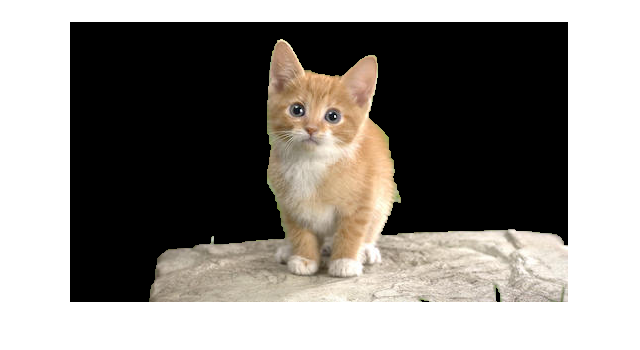
\includegraphics[width = 3in]{cat_out}
  \label{fig:sfig2}
\end{subfigure}



\caption{Foreground Extractions for GMM Model}
\end{figure}

\begin{thebibliography}{10}

\bibitem{1} Rother, Carsten, Vladimir Kolmogorov, and Andrew Blake. "Grabcut: Interactive foreground extraction using iterated graph cuts." ACM Transactions on Graphics (TOG) 23.3 (2004): 309-314.
\bibitem{2} Boykov, Yuri Y., and M-P. Jolly. "Interactive graph cuts for optimal boundary \& region segmentation of objects in ND images." Computer Vision, 2001. ICCV 2001. Proceedings. Eighth IEEE International Conference on. Vol. 1. IEEE, 2001.
\bibitem{3} Kolmogorov, Vladimir, and Ramin Zabin. "What energy functions can be minimized via graph cuts?." Pattern Analysis and Machine Intelligence, IEEE Transactions on 26.2 (2004): 147-159.
\end{thebibliography}
\end{document}